Рассмотрим ход лучей в микроскопе в предположении, что глаз наблюдателя аккомодирован на
бесконечность (рис. \ref{img::6}). Тангенс угла $\varphi_2$ , под которым видно изображение, определяется
соотношением
\
\begin{equation}\label{eq::5}
  \tg \varphi_2 = \frac{l'}{f_2} = \frac{l(\Delta - f_1 - f_2)}{f_1 f_2},
\end{equation}
\
где $l'$ -- размер промежуточного изображения, $l$ -- размер предмета, $\Delta$ -- длина тубуса 
(расстояние между линзами).

\begin{figure}[h]
  \center{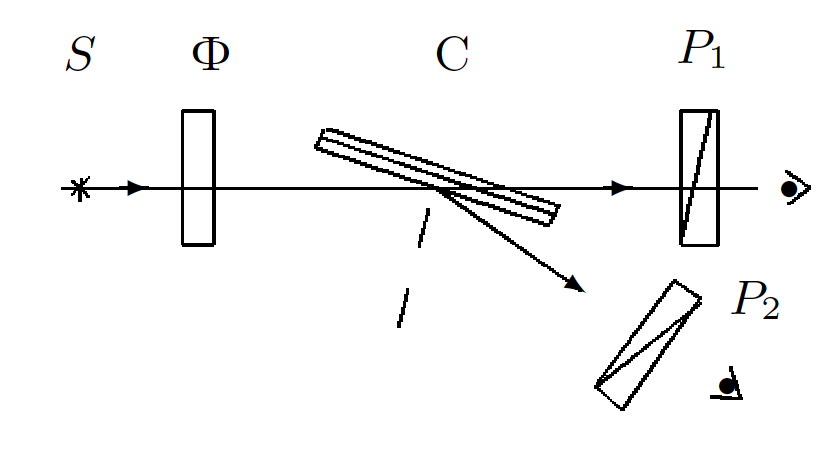
\includegraphics[width=\linewidth]{6.png}}
  \caption{К расчёту увеличения микроскопа}
  \label{img::6}
\end{figure}

При наблюдении предмета невооружённым глазом с расстояния наилучшего зрения $L$ угловой размер 
предмета $l$ равен
\
\begin{equation}
  \tg \varphi_1 = \frac{l}{L}.
\end{equation}
\
Увеличение микроскопа, следовательно, равно

\begin{equation}
  \gamma = \frac{\tg \varphi_2}{\tg \varphi_1} = \frac{l(\Delta - f_1 - f_2)}{f_1 f_2}.
\end{equation}

У всех микроскопов, выпускаемых отечественной промышленностью, длина тубуса равна $\Delta = 16$см.
Следует ещё раз подчеркнуть, что формулы для расчёта увеличения оптических приборов основаны на 
предположении об аккомодации глаза наблюдателя на бесконечность. В этом предположении увеличение 
является объективной характеристикой оптического инструмента. Если глаз наблюдателя изменяет 
аккомодацию, то оптический инструмент должен быть соответственно перефокусирован, и его увеличение 
несколько изменится. В связи с этим часто говорят о субъективном увеличении прибора. Впрочем, 
как правило, разница между субъективным и объективным увеличениями оптического
инструмента оказывается незначительной.

Можно показать, что при аккомодации глаза на расстояние наилучшего зрения $L$ угловое увеличение 
микроскопа $\gamma$ равно линейному $\Gamma$:

\begin{equation}
  \gamma = \Gamma = \frac{l''}{l} = \frac{l'}{l} \cdot \frac{l''}{l'} = 
  \Gamma_{\text{об}} \cdot \Gamma_{\text{ок}}
\end{equation}

С учётом того, что объектив и окуляр микроскопа -- короткофокусные линзы (предмет и промежуточное
изображение лежат практически в фокальных плоскостях объектива и окуляра, а 
$\Delta - f_2 \approx \Delta$), при аккомодации глаза на расстояние наилучшего зрения увеличение 
микроскопа

\begin{equation}
  \gamma = \Gamma = \Gamma_{\text{об}} \cdot \Gamma_{\text{ок}} \approx 
  \frac{\Delta - f_2}{f_1} \cdot \frac{L}{f_2} \approx \frac{\Delta}{f_1} \cdot \frac{L}{f_2}
\end{equation}

Зная увеличение объектива (в стандартных микроскопах оно обычно указано на оправе) и длину тубуса 
(16 см), можно оценить расстояние от объектива до плоскости, в которой следует располагать предмет. 
Обычно это 1-3 см.